\documentclass[aspectratio=169,11pt]{beamer}
\usepackage[T1]{fontenc}
\usepackage{lmodern}
\usepackage{amsmath,amssymb}
\usepackage{booktabs,tabularx}
\usepackage{tikz}
\usetikzlibrary{arrows.meta,positioning}

% ---- Fill in before the talk -------------------------------------------------
\newcommand{\groupletter}{B}
% -----------------------------------------------------------------------------

\definecolor{ink}{HTML}{1B1F24}
\definecolor{muted}{HTML}{5B6470}
\definecolor{accent}{HTML}{2457C5}
\definecolor{soft}{HTML}{E8EEFB}
\definecolor{bad}{HTML}{B3261E}
\definecolor{good}{HTML}{1E7B34}

\setbeamertemplate{navigation symbols}{}
\setbeamercolor{normal text}{fg=ink,bg=white}
\setbeamercolor{frametitle}{fg=ink,bg=white}
\setbeamercolor{structure}{fg=accent}
\setbeamerfont{frametitle}{size=\Large,series=\bfseries}
\setbeamertemplate{frametitle}{\vspace{0.6em}\insertframetitle\par\vspace{-0.2em}{\color{accent}\rule{2.2em}{2pt}}}
\setbeamertemplate{itemize items}{\color{accent}\textbullet}
\setbeamertemplate{footline}{\hfill{\color{muted}\scriptsize\insertframenumber/\inserttotalframenumber}\hspace{1em}\vspace{0.6em}}

\newcommand{\act}[1]{\texttt{#1}}
\newcommand{\acro}[1]{\vfill{\color{muted}\scriptsize #1}}
\newcommand{\LTLG}{\mathbf{G}}
\newcommand{\LTLX}{\mathbf{X}}
\newcommand{\LTLY}{\mathbf{Y}}

\begin{document}

% 1 ---------------------------------------------------------------------------
\begin{frame}[plain]
\vspace{2.2em}
{\color{accent}\small\bfseries CS 3892 \quad Group \groupletter \quad Topic 8: formal models of agentic AI}\\[0.8em]
{\LARGE\bfseries Model Checking MCP-Style Tool-Using Agents}\\[0.5em]
{\large\color{muted} How accurate are LLM-written models, and do their attack traces reproduce?}\\[2em]
{\large Teo Kitanovski \quad Connor Brugger \quad Xiaodi Shao}\\[0.4em]
{\small\color{muted} Project proposal, 29 September 2026}\\[0.4em]
{\small\ttfamily github.com/ConnorBrug/mcp-agent-verification}
\acro{MCP: Model Context Protocol, the standard interface between an LLM agent and its tools.
LLM: large language model.}
\end{frame}

% 2 ---------------------------------------------------------------------------
\begin{frame}{What we are asking}
\centering
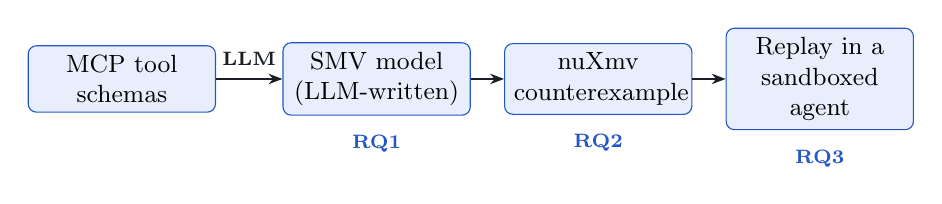
\begin{tikzpicture}[
  box/.style={draw=accent,fill=soft,rounded corners=3pt,minimum height=2.4em,
              text width=6.1em,align=center,font=\small},
  arr/.style={-{Stealth[length=5pt]},thick,color=ink},
  rq/.style={font=\scriptsize\bfseries,color=accent}]
\node[box] (s) {MCP tool\\schemas};
\node[box,right=2.4em of s] (m) {SMV model\\(LLM-written)};
\node[box,right=1.2em of m] (c) {nuXmv\\counterexample};
\node[box,right=1.2em of c] (r) {Replay in a\\sandboxed agent};
\draw[arr] (s) -- node[above=1pt,font=\scriptsize\bfseries]{LLM} (m);
\draw[arr] (m) -- (c);
\draw[arr] (c) -- (r);
\node[rq,below=0.35em of m] {RQ1};
\node[rq,below=0.35em of c] {RQ2};
\node[rq,below=0.35em of r] {RQ3};
\end{tikzpicture}

\vspace{1em}
\raggedright
\begin{itemize}\setlength\itemsep{0.5em}
\item \textbf{RQ1.} How accurately can an LLM translate real MCP tool schemas into a formal
  transition-system model? We compare against hand-written reference models.
\item \textbf{RQ2.} What security violations can we find by model checking the LLM-written models?
\item \textbf{RQ3.} How many of those attack traces reproduce against a sandboxed agent using the
  real tools?
\end{itemize}
\acro{RQ: research question. SMV: the input language of the NuSMV and nuXmv model checkers.}
\end{frame}

% 3 ---------------------------------------------------------------------------
\begin{frame}{The FM half: model, properties, expected verdict}
\begin{columns}[T,onlytextwidth]
\begin{column}{0.44\textwidth}
\footnotesize
\textbf{Model:} a transition system in SMV
\begin{itemize}\setlength\itemsep{0.25em}
\item The LLM picks its next tool action nondeterministically.
\item An attacker input decides whether an untrusted read carries a prompt injection. After
  that, \act{tainted} stays true.
\item Each tool maps to an abstract action, e.g.\ \act{send\_money} $\to$ \act{send\_external}.
\item A guarded variant adds a policy layer that blocks unsafe actions.
\end{itemize}
\end{column}
\begin{column}{0.53\textwidth}
\footnotesize
\textbf{Properties} in LTL ($\LTLG$ always, $\LTLX$ next, $\LTLY$ previous)\\[0.4em]
\begin{tabular}{@{}l@{\;}l@{}}
P1 & $\LTLG(\act{tainted} \rightarrow \LTLG(\act{action} \neq \act{send\_external}))$\\[0.2em]
P2 & $\LTLG(\act{action} = \act{delete} \rightarrow \LTLY(\act{action} = \act{confirm}))$\\[0.2em]
P3 & $\LTLG((\neg\act{privileged} \wedge \LTLX\,\act{privileged}) \rightarrow \act{grant})$
\end{tabular}\\[0.3em]
{\color{muted} P1: no exfiltration after injection. P2: a delete needs a confirm right before it.
P3: no privilege without a grant.}\\[0.9em]
\textbf{Expected verdict}\\[0.2em]
Unguarded model: {\color{bad}\textbf{false}}, with a counterexample trace.\\
Guarded model: {\color{good}\textbf{true}}.\\
LLM-written model: the same verdict as its reference.\\[0.9em]
\textbf{Tool:} nuXmv 2.2.0, BDD engine. NuSMV is the fallback.
\end{column}
\end{columns}
\acro{FM: formal methods. LTL: linear temporal logic. BDD: binary decision diagram.}
\end{frame}

% 4 ---------------------------------------------------------------------------
\begin{frame}[fragile]{Toy run: nuXmv on our two reference models}
\footnotesize
\texttt{\$ make check}\vspace{-0.4em}
\begin{verbatim}
== agent_unguarded
  COUNTEREXAMPLE  G (action = delete ->  Y action = confirm)
  COUNTEREXAMPLE  G (tainted ->  G action != send_external)
  COUNTEREXAMPLE  G ((!privileged &  X privileged) -> grant)
== agent_guarded
  HOLDS           G (tainted ->  G action != send_external)
  HOLDS           G (action = delete ->  Y action = confirm)
  HOLDS           G ((!privileged &  X privileged) -> grant)
\end{verbatim}
\vspace{-0.2em}
\begin{columns}[T,onlytextwidth]
\begin{column}{0.5\textwidth}
\textbf{P1 counterexample} (unguarded model)\\[0.3em]
\begin{tabular}{@{}cll@{}}
\toprule
step & \act{action} & \act{tainted}\\
\midrule
0 & \act{send\_external} & false\\
1 & \act{read\_untrusted} (injected) & false\\
2 & {\color{bad}\act{send\_external}} & {\color{bad}true}\\
\bottomrule
\end{tabular}
\end{column}
\begin{column}{0.46\textwidth}
\vspace{1.2em}
At step 1 the agent reads injected content. At step 2 it sends data out while tainted, which
violates P1.\\[0.5em]
{\color{muted}Our parser turns each trace into JSON, the input format for sandbox replay (RQ3).}
\end{column}
\end{columns}
\acro{JSON: JavaScript Object Notation, a plain-text data format.}
\end{frame}

% 5 ---------------------------------------------------------------------------
\begin{frame}{The AI half and the data}
\small
\textbf{AI half, in one sentence.} Mainly FM4AI: the tool-using LLM agent is the subject we model
and check. An LLM is also the instrument (AI4FM) that writes the models, and RQ1 measures how well.

\vspace{0.7em}
\begin{columns}[T,onlytextwidth]
\begin{column}{0.48\textwidth}
\textbf{AgentDojo} (ETH Zurich, NeurIPS 2024, MIT license)
\begin{itemize}\setlength\itemsep{0.1em}
\item Simulated tool environments with prompt-injection attacks.
\item 4 suites: 74 tools, 97 user tasks, 35 injection tasks.
\item Also our sandbox for RQ3. Loaded on 27 Sep (v0.1.35).
\end{itemize}
\end{column}
\begin{column}{0.48\textwidth}
\textbf{MCP reference servers} (official repository)
\begin{itemize}\setlength\itemsep{0.1em}
\item The fetch, filesystem, and git servers: 27 tools.
\item \act{fetch} is an untrusted read and can leak data through its URL.
\item Cloned on 27 Sep at commit \texttt{f46d957}.
\end{itemize}
\end{column}
\end{columns}

\vspace{0.7em}
\textbf{Scope:} 5 scenarios, one hand-written reference model each, 10 LLM-written models each
(50 total), 3 properties.
\acro{FM4AI: formal methods for AI. AI4FM: AI for formal methods.}
\end{frame}

% 6 ---------------------------------------------------------------------------
\begin{frame}{Success criterion, and what a negative result looks like}
\small
\renewcommand{\arraystretch}{1.4}
\begin{tabularx}{\textwidth}{@{}l>{\raggedright\arraybackslash}X>{\raggedright\arraybackslash}X@{}}
\toprule
 & \textbf{Success if} & \textbf{A negative result means} \\
\midrule
RQ1 & Verdict agreement VA $\geq 0.8$ and false-safe rate FS $\leq 0.1$ over the 50 models
    & LLM-written models need human review before anyone trusts their verdicts \\
RQ2 & Each property violated in $\geq 3$ of 5 scenarios, and $\geq 70\%$ of violations confirmed
      by the reference model
    & Checking LLM-written models mostly finds translation errors, not attacks \\
RQ3 & Counterexample traces reproduce more often than random action sequences ($p < 0.05$)
    & The abstraction is too coarse to predict how real agents fail \\
\bottomrule
\end{tabularx}

\vspace{0.6em}
We fix these thresholds before generating any model. A negative result is still worth reporting,
because it tells people who want LLMs to write formal models where that currently breaks.
\acro{VA: share of properties where the LLM-written model gets the same verdict as its reference.
FS: share of real violations the LLM-written model reports as safe.}
\end{frame}

% 7 ---------------------------------------------------------------------------
\begin{frame}{Who does what, and the likeliest failure}
\small
\begin{columns}[T,onlytextwidth]
\begin{column}{0.47\textwidth}
\textbf{Team}\\[0.3em]
Teo Kitanovski\\
{\color{muted}\footnotesize reference models, nuXmv runs (RQ2)}\\[0.3em]
Connor Brugger\\
{\color{muted}\footnotesize LLM generation pipeline (RQ1)}\\[0.3em]
Xiaodi Shao\\
{\color{muted}\footnotesize sandbox replay (RQ3)}\\[0.8em]
\textbf{Milestone, 12 Nov}\\
{\footnotesize All 50 models checked, RQ1 and RQ2 numbers, scripted replay demo.}\\[0.8em]
{\scriptsize\ttfamily github.com/ConnorBrug/mcp-agent-verification}
\end{column}
\begin{column}{0.50\textwidth}
\footnotesize
\textbf{Likeliest failure.} A trace step like \act{send\_external} does not say which tool to
call or with what arguments, and a real agent may ignore an injection for unrelated reasons.
RQ3 could come out near zero without telling us anything.\\[0.6em]
\textbf{Fallback.} We replay traces two ways. In scripted replay we issue the concrete tool calls
ourselves. In agent-driven replay we plant only the injection. If agent-driven replay costs too
much, we run it on a fixed subset.\\[0.6em]
\textbf{Second risk.} LLM-written models fail to parse. We give the LLM a fixed interface template
and allow 3 repair rounds using nuXmv's error messages.
\end{column}
\end{columns}
\end{frame}

\end{document}
